
%==========================================================================

\begin{frame}[fragile]

  {\Huge Organizational}

  \vspace{15pt}

  \textbf{Content:}
  \begin{itemize}
    \item Kokkos User Group @ HPSF Conference '26 (US)
    \item Save the Date
    \item Mailing Lists
  \end{itemize}

\end{frame}

%==========================================================================

\begin{frame}[fragile]{KUG 2026 Content Available}


\begin{itemize}
\item Videos are online
  \begin{itemize}
  \item Browse the \href{https://hpsf2026.sched.com/overview/type/Kokkos+Project+Meeting}{agenda with slides uploaded and recordings}
  \item Playlist with all the presentations available on \href{https://youtube.com/playlist?list=PLRKq_yxxHw28Ttz9noQiGQglDlZhUFHJ4&si=v-O6KetKLGRQ4h7V}{HPSF's YouTube Channel}
  \end{itemize}
\item Checkout the trip report on our blog \url{https://kokkos.org/blog/2026-03-KUG-report/}
\end{itemize}

\end{frame}

%==========================================================================

\begin{frame}[fragile]{Save The Date}

\textbf{KUG 2027 @ HPSFCon}
\begin{itemize}
\item April 12th - 16th in Montreal Canada
\item Save the date website: \url{https://events.linuxfoundation.org/hpsf-conference/}
\item Call for submissions expected mid September
\end{itemize}

\vspace{5pt}
\textbf{Kokkos Tutorial @ SC26}
\begin{itemize}
\item November 15th-20th Chicago, IL (exact date tbd)
\item Beginner tutorial with hands-on
\item Let your colleagues know!
\end{itemize}
\end{frame}

%==========================================================================

\begin{frame}[fragile]{Citing Kokkos - Help us track the impact of Kokkos}

\begin{itemize}
\item Ensure reproducibility
  \begin{itemize}
  \item Version-specific citations for Core and Kernels since 5.0
  \item Format: \emph{Kokkos Core v5.2.0, DOI: 10.5281/zenodo.21648054}
  \item See \href{https://kokkos.org/about/releases/}{release page} to find the specific DOI for the version you used
  \end{itemize}
\item In addition to that, please also cite relevant papers describing the component of the Ecosystem you used
\end{itemize}

Visit \url{https://kokkos.org/citing-kokkos/}

\end{frame}

%==========================================================================

\begin{frame}[fragile]{Tea-Time Webinar Series}

\begin{columns}
\column{0.5\textwidth}
\begin{itemize}
\item On the 3rd Wednesday of the month at 4 PM Paris time (usually 10 AM Eastern, 8 AM Mountain, 11 PM Tokyo time)
\item Find the playlist on \href{https://youtube.com/playlist?list=PLRKq_yxxHw2-Dkc4rEo8s-b3uaxJfuavA&si=BTBwI65FpP7B08uw}{HPSF YouTube channel}
\item Reach out if you would like to get invited to speak
\end{itemize}

\column{0.5\textwidth}
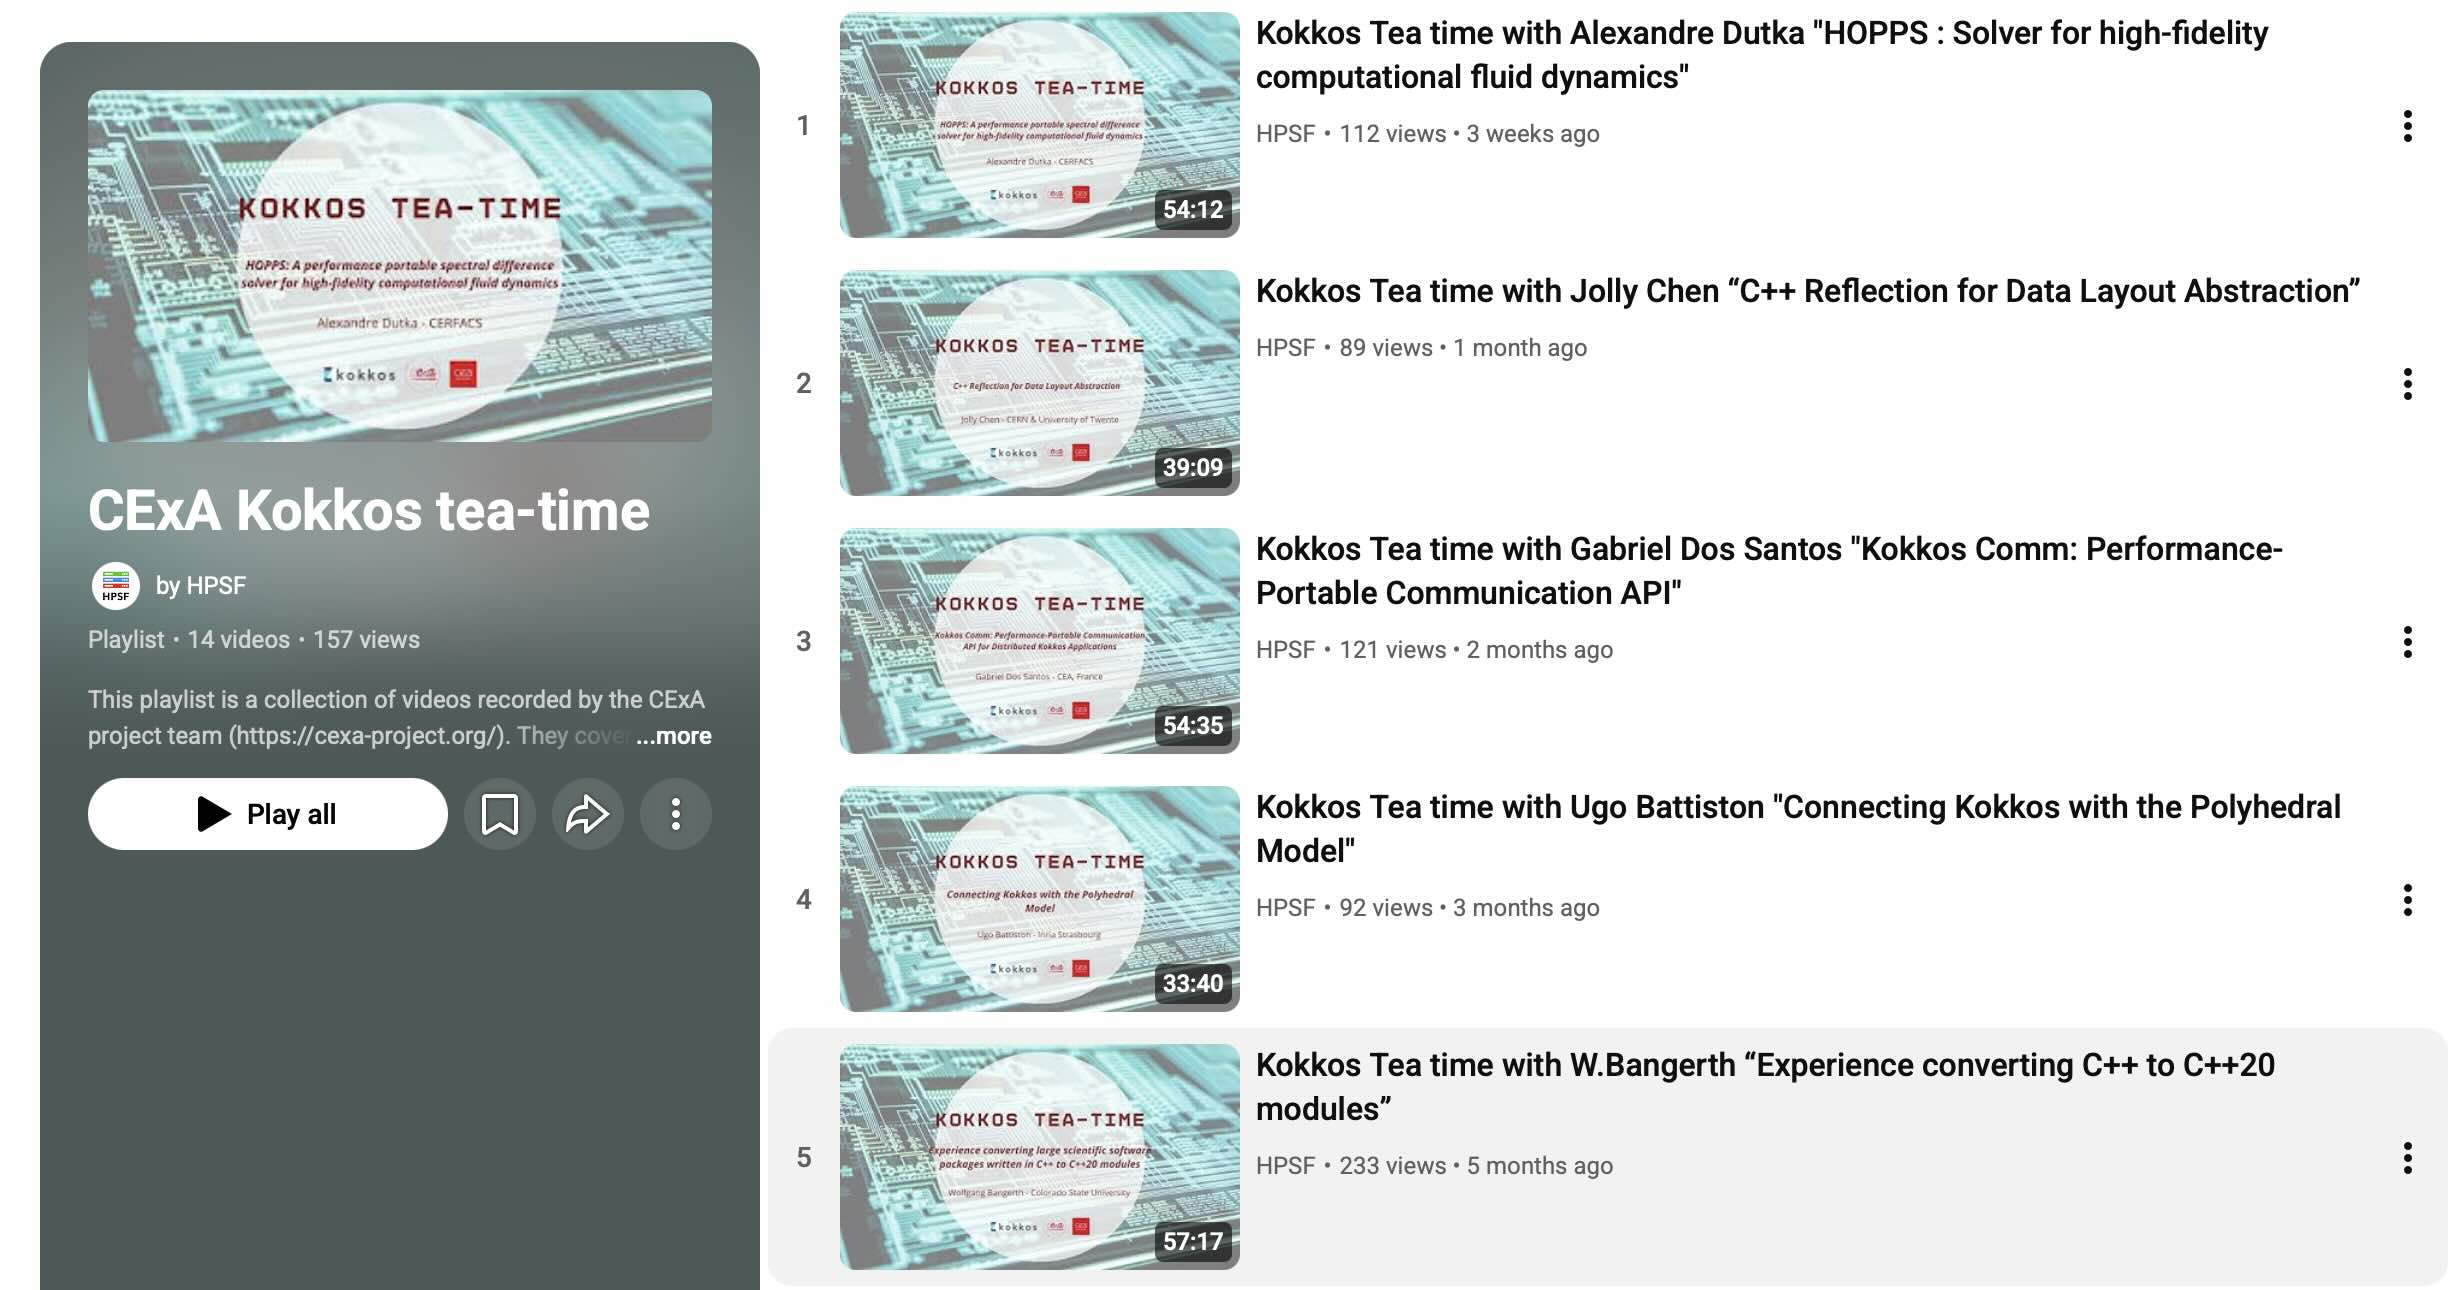
\includegraphics[width=\linewidth]{5_1/kokkos-tea-time-playlist.jpg}
\end{columns}

%\begin{block}{Next session scheduled for tomorrow}
%\emph{Parthenon – a performance portable block-structured adaptive mesh refinement framework}
%by Philipp Grete
%\end{block}

Visit \url{https://kokkos.org/community/tea-time/}

\end{frame}

%==========================================================================

\begin{frame}[fragile]{Roadmap: Deprecation Clean-up}

\begin{block}{Kokkos 5.2: Major Removal}
   Most \texttt{KOKKOS\_ENABLE\_DEPRECATED\_CODE\_4} paths has been \textbf{removed}.
\end{block}

\begin{alertblock}{Final Removal in 5.3}
These remain in 5.2 but will be removed in 5.3:
\begin{description}
    \item[\texttt{MemoryManaged}] $\rightarrow$ Use \texttt{MemoryTraits<>}
    \item[\texttt{View::HostMirror}] $\rightarrow$ Use \texttt{View::host\_mirror\_type}
\end{description}
\end{alertblock}

\begin{itemize}
    \item \textit{Note: Version 5.3 will have zero exceptions for 4.x legacy code.}
\end{itemize}

\end{frame}

%==========================================================================

\begin{frame}[fragile]{Legacy View Removal (Kokkos 5.3)}

\begin{alertblock}{Final Transition}
The legacy \texttt{View} implementation will be removed in 5.3.
\end{alertblock}

\begin{itemize}
    \item \textbf{Status:} \texttt{std::mdspan}-based \texttt{View} has been the default since 5.0.
    \item \textbf{Contingency Flag Removal:} \texttt{-DKokkos\_ENABLE\_IMPL\_VIEW\_LEGACY=ON} will no longer be available.
\end{itemize}

\vfill

\begin{block}{Are you still using the legacy implementation?}
\centering
\textbf{Please reach out to the team via GitHub or Slack!} \\
We need to address any blocking bugs or regressions before 5.3.
\end{block}

\end{frame}

%==========================================================================

\begin{frame}[fragile]{4.7 End of Life}
\vspace{1.5cm}
\begin{center}
   \textbf{Extended support for 4.7 has reached its end.}
\end{center}
\end{frame}

%==========================================================================

% Examples

% note: always keep the [fragile] for your frames!

%\begin{frame}[fragile]{Example list}
%  \begin{itemize}
%      \item Item 1
%      \item Item 2 with some \texttt{code}
%      \begin{itemize}
%        \item Sub-item 2.1
%        \item Sub-item 2.2
%      \end{itemize}
%  \end{itemize}
%\end{frame}

%\begin{frame}[fragile]{Example code}
%    \begin{code}[keywords={std}]
%        #include <iostream>
%
%        int main() {
%            std::cout << "hello world\n";
%        }
%    \end{code}
%\end{frame}

%\begin{frame}[fragile]{Example table}
%    \begin{center}
%        \begin{tabular}{l|l}
%            a & b \\\hline
%            c & d
%        \end{tabular}
%    \end{center}
%\end{frame}

%==========================================================================

